\documentclass{overview}
\title{Calculus Overview - Integrate}

\begin{document}
\maketitle

\section{Identities}
\begin{equation}
	\arcsin t = \arctan \frac{t}{\sqrt{1-t^2}} = 2 \arctan \frac{t}{1+\sqrt{1-t^2}}
	\label{eq:ArcSinToArcTanByHalfAngle}
\end{equation}
\begin{equation}
	\arctan t = \arcsin \frac{t}{\sqrt{1+t^2}} 
\end{equation}
\begin{equation}
	 (x-a)(b-x) = \left(\frac{b-a}{2}\right)^2 - \left(x-\frac{a+b}{2}\right)^2
	 \label{eq:XMinusAXMinusB}
\end{equation}
\begin{equation}
	\frac{1}{1-\sin x} = \frac{1+\sin x}{\cos^2 x} =
	\sec^2 x + \frac{\sin x}{\cos^2 x}
\end{equation}
\begin{equation}
	\frac{1}{1+\cos x} = \frac{1-\cos x}{\sin^2 x} =
	\csc^2 x - \frac{\cos x}{\sin^2 x}
\end{equation}
\begin{equation}
	\frac{1-\sin x}{\cos x} = \frac{\cos x}{1+\sin x} 
\end{equation}
\[
	\text{Above absolute value} = \sqrt{\frac{1-\sin x}{1+\sin x}}
\] 
\begin{equation}
	\frac{1-\cos x}{\sin x} = \frac{\sin x}{1+\cos x}= \tan \frac{x}{2}
\end{equation}

\section{Basic Integrations}
\[
	\begin{array}{c|c}
		\begin{aligned}
			\int \frac{1}{a^2 + x^2} \dd x &= \frac{1}{a} \arctan \frac{x}{a} \\
			\int \frac{1}{a^2 - x^2} \dd x &= \frac{1}{2a} \ln \left| \frac{a+x}{a-x} \right| \\
																		 &= \frac{1}{a} \ath \frac{x}{a} \\
																		 &\quad\text{(when } |x| < |a| \text{)} \\
			\int \frac{1}{\sqrt{a^2 - x^2}} \dd x &= \arcsin \frac{x}{a} \\
			\int \frac{1}{\sqrt{a^2 + x^2}} \dd x &= \ln( x + \sqrt{a^2 + x^2}) \\
																		 &= \ash \frac{x}{|a|} +C'\\
			\int \frac{1}{\sqrt{x^2 - a^2}} \dd x &= \ln \left| x + \sqrt{x^2 - a^2} \right| \\
																		 &= \ach \frac{x}{|a|} +C' \\
																		 &\quad\text{(when } x > |a| \text{)} \\
		\end{aligned} &
		\begin{aligned}
			\int \tan x \dd x &= -\ln|\cos x| \\
			\int \cot x \dd x &= \ln|\sin x| \\
			\boxed{ \int \sec x \dd x} &= \ln|\sec x + \tan x| \\
			\boxed{\int \csc x \dd x} &= \ln|\csc x - \cot x| \\
			\int \sec^2 x \dd x &= \tan x \\
			\int \csc^2 x \dd x &= -\cot x \\
			\int \sec x \tan x \dd x &= \sec x \\
			\int \csc x \cot x \dd x &= -\csc x \\
		\end{aligned}
	\end{array}
\] 

Especially, we have
\[
	\int \frac{1}{\sqrt{1+x^2}} \dd x = \ln(x + \sqrt{1+x^2}) = \ash x + C
\] 
and
\[
	\int \frac{1}{(1+x^2)^{3/2}} \dd x = \frac{x}{\sqrt{1+x^2}} + C
\] 

\subsection{Integrals Involving Square Roots}
The area of a circle segment with radius $a$ 
\[
	\begin{aligned}
	\int \sqrt{a^2 - x^2} \dd x 
	&= \frac{x}{2} \sqrt{a^2 - x^2}
	+ \frac{a^2}{2} \arcsin \frac{x}{a} + C \\
	&=\frac{1}{2} xh + \frac{a^2}{2}\theta
	\end{aligned}
	% TODO: add diagram
\] 
and other forms: (can remember by considering $\sin \to \sh$)
\[
\begin{aligned}
	\int \sqrt{x^2 + a^2} \dd x &= \frac{x}{2} \sqrt{x^2 + a^2}
	+ \frac{a^2}{2} \ln( x + \sqrt{x^2 + a^2}) + C \\
	\int \sqrt{x^2 - a^2} \dd x &= \frac{x}{2} \sqrt{x^2 - a^2}
	- \frac{a^2}{2} \ln \left| x + \sqrt{x^2 - a^2} \right| + C \\
\end{aligned}
\] 

Since \eqref{eq:XMinusAXMinusB} holds, we have
\[
	\int \frac{1}{\sqrt{(x-a)(b-x)}} \dd x = \arcsin \frac{2x - a - b}{b - a}
	= \arcsin \frac{x-a-b+x}{x-a+b-x}
\]
also we can rewrite it using \eqref{eq:ArcSinToArcTanByHalfAngle} as
\[
	\int \frac{1}{\sqrt{(x-a)(b-x)}} \dd x = 2 \arctan \sqrt{\frac{x-a}{b-x}}
\]
especially when $a=0$ we have
\[
	\int \frac{1}{\sqrt{x(b-x)}} \dd x = \arcsin \frac{2x-b}{b} = 2 \arctan \sqrt{\frac{x}{b-x}}
\]

\subsection{Integrals Involving Trigonometric Functions}

% TODO: show why equal
Using tringleometric identities, we can derive the following result:
\[
	\int \sec x \dd x = \ln|\sec x + \tan x| = \ath(\sin x) + C
\] 
and
\[
\int \csc x \dd x = \ln|\csc x - \cot x| = -\ath(\cos x) + C
\] 
when $k\pi < x < (k+1 / 2)\pi$, we have
\[
	\int \csc x \dd x = \ln|\csc x - \cot x| = \ln \left|\tan \frac{x}{2}\right| + C
\] 

For trigonometric squared on denominator, in general we have (when $a ^2+ b^2 > 0$)
\[
	\begin{aligned}
	\int \frac{\dd x}{a^2 \sin^2 x + b^2 \cos^2 x}
	&= \int \frac{\sec^2 x \dd x}{a^2 \tan^2 x + b^2} \\
	&= \int \frac{\dd (\tan x)}{a^2 (\tan x)^2 + b^2} \\
	&= \frac{1}{a} \int \frac{\dd a \tan x}{(a \tan x)^2 + b^2} \\
	&= \frac{1}{a b} \arctan \frac{a \tan x}{b} + C
		\end{aligned}
\] 

\subsection{Useful Integral Results}

\subsubsection{$(t^2 + a^2) ^{-n}$ Integrals}
\[
	I_n = \int \frac{1}{(t^2 + a^2)^n} \dd t
\]
then
\[
	I_n = \frac{1}{2a^2 (n-1)} \left[\frac{t}{(t^2 + a^2)^{n-1}} + (2n - 3) I_{n-1} \right]
\] 
\begin{proof}
	\[
		\begin{aligned}
			a^2 I_n 
			&= \int \frac{a^2 + t^2 - t^2}{(t^2 + a^2)^n} \dd t \\
			&= \int \frac{1}{(t^2 + a^2)^{n-1}} \dd t - \int \frac{t^2}{(t^2 + a^2)^n} \dd t \\
			&= I_{n-1} - \frac{1}{2} \int \frac{t\dd t^2}{(t^2 + a^2)^n} \\
			&= I_{n-1} - \frac{1}{2(1-n)} \int t\dd \frac{1}{(t^2 + a^2)^{n-1}} \\
		\end{aligned}
	\]
	multiply both sides by $2(n-1)$, then use integration by parts on the last term
	\[
		\begin{aligned}
			2(n-1) a^2 I_n
			&= 2(n-1) I_{n-1} + \frac{t}{(t^2 + a^2)^{n-1}} - \int \frac{\dd t}{(t^2 + a^2)^{n-1}} \\
			&= (2n - 3) I_{n-1} + \frac{t}{(t^2 + a^2)^{n-1}} \\
		\end{aligned}
	\] 
\end{proof}
In fact, this equation is hard to remember, what we need to remember is the
technique to derive it, first split the numerator into two parts, then use
integration by parts.
\begin{example}
	\[
		\begin{aligned}
			\int \frac{1}{(1+x^2)^2} \dd x
			&= \int \frac{1+x^2 - x^2}{(1+x^2)^2} \dd x \\
			&= \int \frac{1}{1+x^2} \dd x - \int \frac{x^2}{(1+x^2)^2} \dd x \\
			&= \arctan x + \frac{1}{2} \int x \dd \frac{1}{1+x^2} \\
			&= \arctan x + \frac{x}{2(1+x^2)} - \frac{1}{2} \int \frac{\dd x}{1+x^2} \\
			&= \frac{1}{2}\left(\arctan x + \frac{x}{1+x^2}\right) + C
		\end{aligned}
	\] 
\end{example}

\subsubsection{Sine and Cosine Powers}
\[
	\int \sin^n x \dd x = -\frac{1}{n} \sin^{n-1} x \cos x
	+ \frac{n-1}{n} \int \sin^{n-2} x \dd x
\]
\subsubsection{Trigonometric results}

Those results may be hard to derive during an exam, so it is better to
remember them.

\[
	\int \sec^{3}x \dd x = \frac{1}{2} \sec x \tan x + \frac{1}{2} \ln|\sec x + \tan x| + C
\] 
Tips to remember: is the mean of $\int \sec x \dd x$ and $\dd (\sec x) / \dd x$.
Don't forget
\[
	\frac{\dd}{\dd x} \sec x = \sec x \tan x
\] 

\begin{proof}
	\[
		\begin{aligned}
		\int \sec^3 x \dd x
		&= \int \sec x \cdot \sec^2 x \dd x \\
		&= \int \sec x \dd (\tan x) \\
		&= \sec x \tan x - \int \sec x \tan^2 x \dd x \\
		&= \sec x \tan x - \int \sec x (\sec^2 x - 1) \dd x \\
		&= \sec x \tan x - \int \sec^3 x \dd x + \int \sec x \dd x \\
		\Rightarrow 2 \int \sec^3 x \dd x
		&= \sec x \tan x + \ln|\sec x + \tan x| + C
		\end{aligned}
	\]
\end{proof}

\[
	\begin{aligned}
	\int \frac{1}{1+\cos x} \dd x
	&= \frac{1}{2} \int \sec^2 \frac{x}{2} \dd x \\
	&= \tan \frac{x}{2} + C \\
	&= -\cot x + \csc x + C \\
	\end{aligned}
\] 
\[
	\begin{aligned}
	\int \frac{1}{1+\sin x} \dd x
	&= \int \frac{1-\sin x}{\cos^2 x} \dd x \\
	&= \int \sec^2 x \dd x + \int \frac{\dd \cos x}{\cos^2 x} \\
	&= \tan x - \sec x + C \\
	\end{aligned}
\] 

\section{Techniques of Integration}
\subsection{Trigonometric substitutions}
\begin{itemize}
	\item For integrals involving $\sqrt{a^2 - x^2}$, use $x = a \sin t$.
	\item For integrals involving $\sqrt{a^2 + x^2}$, use $x = a \tan t$.
	\item For integrals involving $\sqrt{x^2 - a^2}$, use $x = a \sec t$. 
\end{itemize}


\subsection{Trigonometric only functions}

For integrals involving only sine and cosine functions
\[
	\int f(\sin x, \cos x) \dd x
\] 
we can use the following strategies:
\begin{itemize}
	\item If $f(-\sin x, \cos x) = -f(\sin x, \cos x)$,  $f$ is odd in $\sin x$, 
		let $t = \cos x$
	\item If $f(\sin x, -\cos x) = -f(\sin x, \cos x)$,  $f$ is odd in $\cos x$, 
		let $t = \sin x$
	\item If $f(-\sin x, -\cos x) = f(\sin x, \cos x)$,  $f$ is even in both $\sin x$ and $\cos x$, 
		let $t = \tan x$
\end{itemize}
then try to rewrite the integral in terms of $t$.


\subsubsection{Trigonometric Rational Functions}
For integrals involving rational functions of sine and cosine, we can use the
tangent half-angle substitution, let $t = \tan \frac{x}{2}$, then
\[
\int f (\sin x, \cos x)\, dx = \int f {\left ({\frac {2 t} {1 + 
          t^{2}}}, {\frac {1 - t^{2}} {1 + t^{2}}} \right)} {\frac {2\, dt} {1 + t^{2}}}
\]
becomes an integral of rational function.

\subsubsection{Combining Sine and Cosine}
when ask for $I_1=\int \sin^n x \dd x$ and $I_2=\int \cos^n x \dd x$ at the same time,
we can try to combine them, calculate $I_1 + I_2$ and $I_1 - I_2$ separately.
Hoping to get $\sin^2 x + \cos^2 x$
\begin{example}
	\[
		\begin{aligned}
		I_1 &= \int \sin^4 x \dd x \\
		I_2 &= \int \cos^4 x \dd x \\
		\end{aligned}
	\] 
	then
	\[
		\begin{aligned}
		I_1 + I_2 &= \int (\sin^4 x + \cos^4 x) \dd x \\
							&= \int (1 - 2 \sin^2 x \cos^2 x) \dd x \\
							&= x - \frac{1}{2} \int \sin^2 2x \dd x = \cdots
		\end{aligned}
	\]
	and
	\[
		\begin{aligned}
		I_1 - I_2 &= \int (\sin^4 x - \cos^4 x) \dd x \\
							&= \int (\sin^2 x - \cos^2 x)(\sin^2 x + \cos^2 x) \dd x \\
							&= \int \cos 2x \dd x = \frac{1}{2} \sin 2x + C
		\end{aligned}
	\]
\end{example}

\subsection{Integration by parts}
\subsubsection{Tabular Integration}
When we have an integration of the form $\int P(x) e^{ax} \dd x$ or $\int P(x) 
\sin(ax) \dd x$ or $\int P(x) \cos(ax) \dd x$, where $P(x)$ is a polynomial, we
can use tabular integration to speed up the process. For example,
\[
	\int x^2 e^{ax} \dd x
\]
we can set up the table as follows:
\[
	\begin{array}{ccccc}
		\text{Derivatives} & \color{red}x^2 & \color{blue}2x & 2 & 0 \\
		\text{Integrals} & e^{ax} & \color{red}\frac{1}{a} e^{ax} & \color{blue}\frac{1}{a^2} e^{ax} & \frac{1}{a^3} e^{ax} \\
	\end{array}
\]
Then we take the diagonal products, alternating signs:
\[
	\int x^2 e^{ax} \dd x = \color{red}x^2 \cdot \frac{1}{a} e^{ax}
				\color{blue} - 2x \cdot \frac{1}{a^2} e^{ax}
				+ 2 \cdot \frac{1}{a^3} e^{ax} + C
\]
\subsubsection{Determinant Method}
For integrations of the form Exponential times Trigonometric, such as
\[
	\int e^{ax} \sin bx \dd x
\]
although we can use Euler's formula to convert the sine function into complex exponentials,
an quicker trick is 
\[
	\int e^{ax} \sin bx \dd x = \frac{\begin{vmatrix}
			(e^{ax})' & ( \sin bx )' \\
			e^{ax} & \sin bx
	\end{vmatrix}}{a^2 + b^2} + C
\] 
the first row is the derivatives of the two functions, the second row is the
functions themselves. 

Notice: in the determinant, the first column is exponential function. 
\begin{example}
	\[
	\int e^{x} \sin x \dd x = \frac{\begin{vmatrix}
			e^{x} & \cos x \\
			e^{x} & \sin x
	\end{vmatrix}}{1^2 + 1^2} + C
	= \frac{1}{2} e^{x} (\sin x - \cos x) + C
	\] 
\end{example}
	
\subsection{Decomposing}

\subsubsection{Polynomial Division}
\[
	\frac{t^2}{t^2-1}=1+\frac{1}{t^2-1}
\] 
\[
	\frac{1}{1+t} = 1 - \frac{t}{1+t}
\] 
\[
	\begin{aligned}
	\frac{1}{(t^2-1)(1+t)} 
	&= \frac{1}{2}\frac{(1+t)-(t-1)}{(t-1)(t+1)(1+t)} \\
	&= \frac{1}{2}\frac{1}{t^2-1} - \frac{1}{2}\frac{1}{(1+t)^2}
	\end{aligned}
\] 
\[
	\frac{t}{\sqrt{t-1}} = \sqrt{t-1} + \frac{1}{\sqrt{t-1}}
\] 

Numerator rationaliztion:
\[
	\frac{x^2}{1+\sqrt{1-x^2}} = \frac{x^2(1-\sqrt{1-x^2})}{(1+\sqrt{1-x^2})(1-\sqrt{1-x^2})}
	= 1 - \sqrt{1-x^2}
\] 

Divide by same power: (which is hard to spot when first seen)
\[
	\frac{x^2+1}{x^{4}+1} = \frac{1 + \frac{1}{x^2}}{x^2 + \frac{1}{x^2}}
\] 
\begin{example}[divide by same power. 1]
	\[
		\begin{aligned}
		\int \frac{x^2+1}{x^{4}+1} \dd x 
		&= \int \frac{1 + \frac{1}{x^2}}{x^2 + \frac{1}{x^2}} \dd x \\
		&= \int \frac{d(x - \frac{1}{x})}{(x - \frac{1}{x})^2 + 2} \\
		&= \frac{1}{\sqrt{2}} \arctan \frac{x - \frac{1}{x}}{\sqrt{2}} + C
		\end{aligned}
	\]
\end{example}
\begin{example}[divide by same power. 2]
	\[
		\begin{aligned}
			\int \frac{x^2-1}{x^{4}+1} \dd x 
			&= \int \frac{1 - \frac{1}{x^2}}{x^2 + \frac{1}{x^2}} \dd x \\
			&= \int \frac{d(x + \frac{1}{x})}{(x + \frac{1}{x})^2 - 2} \\
			&= \frac{1}{2\sqrt2} \ln \left| \frac{x + \frac{1}{x} - \sqrt{2}}{x + \frac{1}{x} + \sqrt{2}} \right| + C
		\end{aligned}
	\]
\end{example}
\begin{example}[divide by same power. use above]
\[
		\begin{aligned}
				\int \frac{1}{x^{4}+1} \dd x 
				&= \frac{1}{2} \left(\int \frac{x^2+1}{x^{4}+1} \dd x - \int \frac{x^2-1}{x^{4}+1} \dd x\right)
			\end{aligned}
	\] 
\end{example}

\begin{example}
	\[
		\int \frac{1}{1+e^x} \dd x = \int \left( 1 - \frac{e^x}{1+e^x} \right) \dd x
		= x - \ln(1+e^x) + C
	\]
\end{example}

\subsection{Rational Functions}

For integrals involving rational functions, we use partial fraction decomposition in
most cases.

First we need to write the rational function in proper form.

\subsubsection{Undetermined Coefficients Method}

Any proper rational function can be decomposed into sum of simple proper rational functions
\[
	D(x) = \prod_{i=1}^m (x-a_i)^{n_i} \prod_{j=1}^k (x^2 + b_j x + c_j)^{m_j}
	\quad\quad(\text{satisfying }b_j^2 - 4 c_j < 0)
\] 
then we can decompose
\[
	\frac{N(x)}{D(x)} = \sum_{i=1}^m \sum_{r=1}^{n_i} \frac{A_{ir}}{(x-a_i)^r}
	+ \sum_{j=1}^k \sum_{s=1}^{m_j} \frac{B_{js} x + C_{js}}{(x^2 + b_j x + c_j)^s}
\] 
that is, for each linear factor $(x-a_i)^{n_i}$ in the denominator,
we need to include $n_i$ terms in the decomposition and correspondingly $n_i$
undetermined coefficients, and for each quadratic factor $(x^2 + b_j x + c_j)^{m_j}$
in the denominator, we need to include $m_j$ terms in the decomposition and correspondingly
$2 m_j$ undetermined coefficients.
\begin{example}[one linear factor and one repeated linear factor]
	\[
		\frac{3x^2-8x+13}{(x+3)(x-1)^2} = \frac{A}{x+3} + \frac{B}{x-1} + \frac{C}{(x-1)^2}
	\]
\end{example}
\begin{example}[with quadratic factor]
	\[
		\frac{x^{4}+2x^{3}+3x^2+4x+1}{(x+1)(x-1)^2(x^2+1)} =
		\frac{A}{x+1} + \frac{B}{x-1} + \frac{C}{(x-1)^2} + \frac{D x + E}{x^2 + 1}
	\]
\end{example}

Now focus on how to find the undetermined coefficients, instead of reducing to
common denominator and comparing coefficients, we can use Residue method, we
do not proof it here, just give how to use it. (TODO: add proof later)

For non-repeated linear factor $(x-a_i)$ (\underline{Notice: the coefficient of $x$ in
the factor should be 1}) in the denominator, the corresponding
coefficient $A_i$ can be found by
\[
	A_i = \lim_{x \to a_i} \left[\frac{N(x)}{D(x)}(x-a_i)\right]
\]
When the coefficient is not 1, for example $(k x - a_i)$, we need first divide both
numerator and denominator by $k$, then apply the formula above.
	
For repeated linear factor $(x-a_i)^{n_i}$ (Notice: also the coefficient of $x$ 
should be 1) in the denominator, the
corresponding coefficient $A_{i, n_i}$ (the one with highest power) can be found by
\[
	A_{i, n_i} = \lim_{x \to a_i} \left[\frac{N(x)}{D(x)}(x-a_i)^{n_i}\right]
\] 
and the other coefficients can be found by
\[
	A_{i, r} = \frac{1}{(n_i - r)!} \lim_{x \to a_i} \left[ \frac{\dd^{n_i - r}}{\dd x^{n_i - r}}
	\left(\frac{N(x)}{D(x)}(x-a_i)^r\right) \right]
\]

For quadratic factor $(x^2 + b_j x + c_j)$ in the denominator, although we can
find both $B_j$ and $C_j$ by solving two equations, using similar method as above,
but it will involve complex numbers and too much complexity, in that case, it
is better to let $x$ equal to some convenient values to form equations to solve.

Also for some quadratic factors, we can try changing variable to simplify the expression

\subsubsection{Linear numerator divided by quadratic denominator}
For integrals of the form
\[
	\int \frac{B x + C}{ax^2 + b x + c} \dd x
\]
we can try to rewrite the numerator as the derivative of the denominator plus a constant,
\begin{example}
	\[
		\begin{aligned}
		\int \frac{x+5}{x^2 - 6x + 13} \dd x
		&= \frac{1}{2}\int \frac{(2x - 6) + 16}{x^2 - 6x + 13} \dd x \\
		&= \frac{1}{2} \int \frac{\dd (x^2 - 6x + 13)}{x^2 - 6x + 13}
		+ 8 \int \frac{1}{(x-3)^2 + 4} \dd x \\
		&= \frac{1}{2} \ln|x^2 - 6x + 13| + 4 \arctan \frac{x-3}{2} + C
		\end{aligned}
	\]
	
\end{example}

Similarly, for integrals of the form
\[
	\int \frac{A\sin x + B \cos x}{C \sin x + D \cos x} \dd x
\] 
we can try to rewrite the numerator as the derivative of the denominator plus 
multiple of the denominator,
\[
C\sin x + D \cos x = E(A \sin x + B \cos x) + F(A \sin x + B \cos x)'
\] 
\subsection{Euler Substitutions}

TODO: explain how this substitution comes to your mind.

For integrals involving $\sqrt{a x^2 + b x + c}$, we can use Euler substitutions.
\begin{itemize}
	\item When $a > 0$, let $\sqrt{a x^2 + b x + c} = \sqrt{a} x + t$.
	\item When $c > 0$, let $\sqrt{a x^2 + b x + c} = x t + \sqrt{c}$.
	\item When $a < 0$ and $c < 0$, let $\sqrt{a x^2 + b x + c} = (x - x_1) t$,
	where $x_1$ is a root of the quadratic equation $a x^2 + b x + c = 0$.
\end{itemize}
\begin{example}
	\[
		I=\int \frac{\dd x}{x+\sqrt{x^2+ 2x + 2}}
	\]
	Let $\sqrt{x^2 + 2x + 2} = x + t$, then
	\[
		x = \frac{t^2 - 2}{2(1-t)}, \quad
		\quad \dd x = \frac{-2+2t-t^2}{2 (1-t)^2} \dd t
	\] 
	Substituting back into the integral, we have
	\[
		I = \int \frac{\frac{-2+2t-t^2}{2 (1-t)^2} \dd t}{\frac{t^2 - 2}{1-t} + t}
		= \int \frac{-2+2t - t^2}{2(1-t)(t-2)} \dd t
	\]
\end{example}

\section{Definite Integrals}
\subsection{Interval change and representation}
For definite integrals, we can change the interval of integration
\[
	\begin{aligned}
	\int_a^b f(x) \dd x \xlongequal{x = a + b - t} 
	&-\int_b^a f(a + b - t) \dd t \\
		=& \int_a^b f(a + b - x) \dd x \\
		=& \frac{1}{2} \int_a^b [f(x) + f(a + b - x)] \dd x
	\end{aligned}
\] 

Especially when the denominator has part of the numerator, and when we
substitute the variable of same part to symmetric about mid of the interval,
get same terms, this technique can be very useful.

\begin{example} 
	Interval $[0, \frac{\pi}{2}]$, after substitution $x = \frac{\pi}{2} - t$,
	we have  $\sin \to \cos$ and $\cos \to \sin$, get same terms.
	\[
		\begin{aligned}
			\int_0^{\frac{\pi}{2}} \frac{e^{\sin x}}{e^{\sin x} + e^{\cos x}} \dd x
			&= \frac{1}{2} \int_0^{\frac{\pi}{2}} \left[
				\frac{e^{\sin x}}{e^{\sin x} + e^{\cos x}} +
				\frac{e^{\cos x}}{e^{\cos x} + e^{\sin x}}
			\right] \dd x \\
			&= \frac{1}{2} \int_0^{\frac{\pi}{2}} \dd x = \frac{\pi}{4}
		\end{aligned}
	\] 
\end{example}

\begin{example}
	Interval $[-\frac{\pi}{2}, \frac{\pi}{2}]$, after substitution $x = -t$,
	we have  $e^{x} \to e^{-x}$ get similar terms.
	\[
	\begin{aligned}
		\int_{-\frac{\pi}{2}}^{\frac{\pi}{2}} \frac{e^{x} \sin^2 x}{1 + e^{x}} \dd x
		&= \frac{1}{2} \int_{-\frac{\pi}{2}}^{\frac{\pi}{2}} \left[
			\frac{e^{x} \sin^2 x}{1 + e^{x}} +
			\frac{e^{-x} \sin^2(-x)}{1 + e^{-x}}
		\right] \dd x \\
		&= \frac{1}{2} \int_{-\frac{\pi}{2}}^{\frac{\pi}{2}} \sin^2 x \dd x
		= \frac{\pi}{4}
	\end{aligned}
	\] 
\begin{remark}
	for this example, we can also use the property that
	\[
		\frac{e^{x}}{1 + e^{x}} - \frac{1}{2} = \frac{1}{2} \cdot \frac{e^{x} - 1}{e^{x} + 1}
	\] 
	is an odd function, so we can replace the integrand by $\frac{1}{2} \sin^2 x$ directly.
\end{remark}
\end{example}

\begin{theorem}
	When $a=-b$ we have
	\[
		\int_{-a}^{a} f(x) \dd x =  \frac{1}{2} \int_{-a}^{a} [f(x) + f(-x)] \dd x
		= \int_0^{a} [f(x) + f(-x)] \dd x
	\]
\end{theorem}

\begin{example}
	Interval $[0, 1]$, after substitution $x = 1 - t$,
	we have  $e^{x} \to e^{1-x}$ get same terms on denominator.
	\[
		\int_0^1 \frac{x}{e^{x} + e^{1-x}} \dd x
		= \frac{1}{2} \int_0^1 \frac{x + (1-x)}{e^{x} + e^{1-x}} \dd x
	\] 
\end{example}

\begin{example} substitution make square root parts simpler.
	\[
		\int_0^{1} x \sqrt{1-x} \dd x
		= \int_0^{1} (1-x) \sqrt{x} \dd x
		= \int_0^{1} x^{1/2} - x^{3/2} \dd x
		= \frac{4}{15}
	\] 
\end{example}

\begin{theorem}[Inference 1]
	\[
		\int_0^{\frac{\pi}{2}} f(\sin x, \cos x) \dd x = \int_0^{\frac{\pi}{2}} f(\cos x, \sin x) \dd x
	\] 
\begin{proof}
	\[
		\begin{aligned}
		\int_0^{\frac{\pi}{2}} f(\sin x, \cos x) \dd x
		&= \int_0^{\frac{\pi}{2}} f(\sin(\frac{\pi}{2} - x), \cos(\frac{\pi}{2} - x)) \dd x \\
		&= \int_0^{\frac{\pi}{2}} f(\cos x, \sin x) \dd x \\
		\end{aligned}
	\]
\end{proof}
\end{theorem}

\begin{theorem}[Inference 2]
When $f$ is continuous on $[0, \pi]$, then
 \[
	 \int_0^{\pi} x f(\sin x) \dd x 
	 =\frac{\pi}{2} \int_0^{\pi} f(\sin x) \dd x
	 =\pi \int_0^{\frac{\pi}{2}} f(\sin x) \dd x
\] 
\begin{proof}
	\[
		\begin{aligned}
		\int_0^{\pi} x f(\sin x) \dd x
		&= \frac{1}{2}\int_0^{\pi} x f(\sin x) + (\pi - x) f(\sin(\pi - x)) \dd x \\
		&= \int_0^{\pi} \frac{\pi}{2} f(\sin x) \dd x \\
		\end{aligned}
	\]
	and since $\sin x$ is symmetric about $\pi/2$, we have
	\[
		\int_0^{\pi} f(\sin x) \dd x = 2 \int_0^{\frac{\pi}{2}} f(\sin x) \dd x
	\]
\end{proof}

\begin{example}
	\[
		\int_0^{\pi} \frac{x}{2+\sin x} \dd x = \frac{\pi}{2} \int_0^{\pi} \frac{1}{2+\sin x} \dd x
		= \pi \int_0^{\frac{\pi}{2}} \frac{1}{2+\sin x} \dd x
		= \frac{\sqrt3}{9} \pi
	\]
	Ignoring the steps to calculate the last integral.
\end{example}

For functions in form of $f(\sin x, \cos x)$, this formula holds when $f$ is symmetric
about the line $x=\pi/2$, that is, $f(\sin x, \cos x) = f(\sin(\pi - x), \cos(\pi - x))
= f(\sin x, -\cos x)$.
\begin{example}[Inference(f(sin x, cos x))]
	\[
		\int_0^{\pi} x |\cos x| \sin x \dd x = \frac{\pi}{2} \int_0^{\pi} |\cos x| \sin x \dd x
	\] 
\end{example}
\end{theorem}


Since $\int f(x)g(x) \dd x$ can be viewed as using $g(x)$ as weight function
to stretch or compress $f(x)$, in fact for any function $f$ symmetric about mid
of the interval $[a, b]$, the line $x=x_0=(a+b) / 2$, when multiplied by a
linear function $g$ symmetric about the point $(x_0, y_0)$, we can say on average,
the integral are stretched by a factor of $y_0$.
that is, the integral can be represented as
\[
	\int_a^b (kx+m)f(x) \dd x = y_0 \int_a^b f(x) \dd x
\]

\begin{example}
	Since $|\cos x|$ is symmetric about $x=n\pi/2$ on interval $[0, n\pi]$, we have
	\[
		\int_0^{n\pi} x |\cos x| \dd x = \frac{n\pi}{2} \int_0^{n\pi} |\cos x| \dd x
	\] 
\end{example}
\begin{example}
	Since $\sqrt{2x - x^2}$ is symmetric about $x=1$ on interval $[0, 2]$, we have
	\[
		\int_0^{2} x\sqrt{2x-x^2} \dd x
		= \int_0^{2} \sqrt{2x-x^2} \dd x
		= \frac{\pi}{2}
	\] 
\end{example}
\begin{theorem}
	When continuous function $f$ satisfies $f(2T-x) = f(x)$ then
	\[
		\int_0^T x f(x) \dd x = \frac{T}{2} \int_0^T f(x) \dd x
	\] 
\end{theorem}

\begin{theorem}[Inference(Symmetric)]
	If $f$ is continuous, then
	\[
		\begin{aligned}
		\int_{0}^{\frac{\pi}{2}} f(\sin x) \dd x = \int_{\frac{\pi}{2}}^{\pi} f(\sin x) \dd x \\
			\int_{-\frac{\pi}{2}}^{\frac{\pi}{2}} f(\sin x) \dd x = \int_{\frac{\pi}{2}}^{\frac{3\pi}{2}} f(\sin x) \dd x \\
			\end{aligned}
			\quad
			\vcenter{\hbox{
			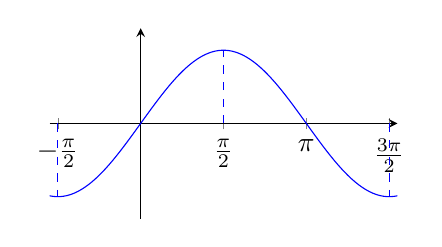
\begin{tikzpicture}
			\begin{axis}[
				axis lines=middle,
				ymin=-1.3, ymax=1.3,
				domain=-1.1*pi/2:3.1*pi / 2,
				ytick=\empty,
				xtick={-3.14159, -1.5708, 0, 1.5708, 3.14159, 4.71239, 6.28318},
				xticklabels={$-\pi$, $-\frac{\pi}{2}$, $0$, $\frac{\pi}{2}$, $\pi$, $\frac{3\pi}{2}$, $2\pi$},
				samples=100,
				width=6cm,
				height=4cm,
				trig format plots=rad,
			]
			\addplot [blue, ] {sin(x)};
			\addplot+[dashed, blue, ycomb, mark=none] plot coordinates {
				(-pi/2,-1) (pi/2,1) (3*pi/2,-1)
			};
			\end{axis}
			\end{tikzpicture}
		}}
	\] 
\end{theorem}

\subsection{Wallis Formula}
\[
	\int_0^{\frac{\pi}{2}} \sin^n x \dd x =
	\int_0^{\frac{\pi}{2}} \cos^n x \dd x =
	\begin{cases}
		\frac{(n-1)!!}{n!!} \cdot \frac{\pi}{2}, & n \text{ even} \\
		\frac{(n-1)!!}{n!!}, & n \text{ odd}
	\end{cases}
\]

and its generalization
\[
	\int_0^{\frac{\pi}{2}} \sin^m x \cos^n x \dd x =
	\frac{(m-1)!! (n-1)!!}{(m+n)!!} \cdot
	\begin{cases}
		\frac{\pi}{2}, & m, n \text{ all even} \\
		1, & \text{otherwise}
	\end{cases}
\] 
% TODO: add proof

\begin{example}
	some integrals can be converted by trigonometric substitution
	\[
		\int_0^1 x\sqrt{1-x} \dd x
		\xlongequal{x = \sin^2 t}
		= \int_0^{\frac{\pi}{2}} 2 \sin^3 t \cos^2 t \dd t
		= 2 \cdot \frac{2!! \cdot 1!!}{5!!} = \frac{4}{15}
	\] 
	
\end{example}
\section{Common Mistakes}
\subsection{Piceewise functions}
In general, when integrating piecewise functions, we need to make sure to
the integral of a piecewise function continuous at the boundaries.

\end{document}
